\documentclass{report}

\input{templates/preamble}
\input{templates/macros}
\input{templates/letterfonts}

\title{\Huge{Relativistic Quantum Waves (Klein-Gordon Equation)}\\ And expanding to the Dirac equation }
\author{\Huge{Marcus Allen Denslow}}
\date{2025-11-14}

\begin{document}

\maketitle
\newpage% or \cleardoublepage
% \pdfbookmark[<level>]{<title>}{<dest>}
\pdfbookmark[section]{\contentsname}{toc}
\tableofcontents
\pagebreak


\chapter{Deriving the KG Equation}
\section{The Strategy: Combining Relativity and Quantum Mechanics}
The goal is to derive a relativistic wave equation that respects both special relativity and quantum mechanics. The strategy is to:
\begin{enumerate}
    \item Start with Einstein's relativistic energy-momentum relation
    \item Replace classical quantities (energy, momentum) with quantum operators
    \item Apply these operators to a wavefunction $\psi$
\end{enumerate}
This "double derivative" approach (squaring the energy) will give us a second-order differential equation.

\dfn{Relativity: the mass shell (Einstein's energy-momentum relation)}{
	Einstein showed that energy and momentum are related by:\\
	$\displaystyle E^2 = (pc)^2 + (mc^2)^2$\\
	Rearranging in four-vector notation:
	$\displaystyle p \cdot p = (mc)^2 \to (mc)^2 = \left( \frac{E}{c} \right)^2 - p^2_{x} - p^2_{y} - p^2_{z}$\\
	This is called the \textbf{mass shell} --- it's a constraint that relates energy and momentum for a particle with mass $m$.
}

\dfn{Quantum: energy and momentum operators}{
In quantum mechanics, we promote classical observables to operators that act on wavefunctions. From the Schr\"{o}dinger equation and de Broglie relations:
\begin{itemize}
    \item Energy operator: $\hat{E} = i\hbar \frac{\partial}{\partial t}$
    \item Momentum operator: $\hat{p} = -i\hbar \nabla$
\end{itemize}
To use these in Einstein's energy-momentum relation, we need to square them. When we square an operator, we apply it twice:\\
\\
\textbf{Energy term:}

\begin{equation}
    \left( \frac{E}{c} \right)^2 \to \left( \frac{\hat{E}}{c} \right)^2 = \left( \frac{i\hbar}{c} \frac{ \partial }{ \partial t }  \right)^2 = - \frac{\hbar^2}{c^2}\frac{ \partial^2 }{ \partial t^2 } 
\end{equation}


\textbf{Momentum terms:}

\begin{equation}
	\hat{p}_{x} = -i\hbar\frac{ \partial }{ \partial  x} \to -p^2_{x} \to \hbar^2\frac{ \partial^2 }{ \partial x^2 } 
\end{equation}


\begin{equation}
    \text{Likewise: } -p^2_{y} \to \hbar^2\frac{ \partial^2 }{ \partial y^2 } \quad \text{ and } \quad -p^2_{z} \to \hbar^2\frac{ \partial^2 }{ \partial z^2 } 
\end{equation}
}


\section{Substituting Operators into Einstein's Relation}
Now we substitute the quantum operators into the relativistic mass shell equation. Remember, these operators will act on a wavefunction $\psi$:
\begin{align*}
	(mc)^2 &= \left( \frac{E}{c} \right)^2 - p^2_{x} - p^2_{y} - p^2_{z} \\
	(mc)^2 &= -\frac{\hbar^2}{c^2}\frac{\partial^2}{\partial t^2} + \hbar^2\frac{\partial^2}{\partial x^2} + \hbar^2\frac{\partial^2}{\partial y^2} + \hbar^2\frac{\partial^2}{\partial z^2}
.\end{align*}
Dividing through by $\hbar^2$ and rearranging:
\begin{equation}
	\frac{1}{c^2}\frac{\partial^2}{\partial t^2} - \frac{\partial^2}{\partial x^2} - \frac{\partial^2}{\partial y^2} - \frac{\partial^2}{\partial z^2} + \left(\frac{mc}{\hbar}\right)^2 = 0
\end{equation}

\section{The Klein-Gordon Equation!}
We've done it! This is the \textbf{Klein-Gordon equation} --- the first successful attempt at a relativistic quantum wave equation.\\
\\
Operating on a wavefunction $\psi$:
\begin{equation}
	\left[\frac{1}{c^2}\frac{\partial^2}{\partial t^2} - \frac{\partial^2}{\partial x^2} - \frac{\partial^2}{\partial y^2} - \frac{\partial^2}{\partial z^2} + \left(\frac{mc}{\hbar}\right)^2\right] \psi = 0
\end{equation}
\textbf{Key features:}
\begin{itemize}
    \item Second-order in both time and space (treats them equally --- relativistic!)
    \item Reduces to Schr\"{o}dinger equation in the non-relativistic limit
    \item Contains the mass $m$ explicitly
\end{itemize}


\section{Compact Notation: Laplacian}
We can write the spatial derivatives more compactly using the Laplacian operator:

\begin{equation}
    \nabla^2 = \frac{ \partial^2 }{ \partial x^2 } + \frac{ \partial^2 }{ \partial y^2 } + \frac{ \partial^2 }{ \partial z^2 } 
\end{equation}


Note the sign: in our equation we have $-\nabla^2$ because of the minus signs in the original expression.\\
\\
Substituting this into our equation:
\begin{equation}
	\left[\frac{1}{c^2}\frac{\partial^2}{\partial t^2} - \nabla^2 + \left(\frac{mc}{\hbar}\right)^2\right]\psi = 0
\end{equation}
This is cleaner and makes the equation look more symmetric.

\section{Even More Compact: d'Alembertian Notation}
We can make this even more compact by defining two convenient symbols:\\
\\
\textbf{The d'Alembertian operator} (wave operator):

\begin{equation}
	\Box = \frac{1}{c^2}\frac{ \partial^2 }{ \partial t^2 } - \nabla^2
\end{equation}


This is the relativistic generalization of the Laplacian. It's the natural wave operator in spacetime.\\
\\
\textbf{The mass parameter:}

\begin{equation}
   \mu = \frac{mc}{\hbar} 
\end{equation}

This has units of inverse length (like a wavenumber). It represents the "Compton wavenumber" of the particle.
\nt{In natural units where $c = \hbar = 1$, we'd just write $\mu = m$. But we keep factors explicit for clarity.}

With these definitions, the Klein-Gordon equation becomes beautifully simple:
\begin{equation}
	\left[\Box + \mu^2\right]\psi = 0
\end{equation}
This compact form makes it easy to see: it's a wave equation (the $\Box$) with a mass term ($\mu^2$).
\\
\chapter{Four-momentum Eigenstates}
Now that we have the Klein-Gordon equation, what are its solutions? The simplest solutions are plane waves --- states with definite energy and momentum.

\section{Klein-Gordon Plane Wave Solutions}
Just like in non-relativistic quantum mechanics, we look for plane wave solutions. These represent particles with definite four-momentum.

\dfn{Klein-Gordon Plane Wave function}{
	The general form using four-vector notation:

	\begin{equation}
		\psi = A \exp \left( -\frac{i}{\hbar}p \cdot x \right) 
	\end{equation}


	where:
	\begin{alignat*}{2}
		p = \left[E/c, \vec{p}\right] &\quad \text{(four-momentum)} \\
		x = \left[ct, \vec{x}\right] &\quad \text{(four-position)} \\
		A \in \mathbb{C} &\quad \text{(complex amplitude)} \\
		p^{0} = \frac{E}{c} = \pm\sqrt{|\vec{p}|^2 + m^2c^2} &\quad \text{(energy, with } \pm \text{ solutions!)}
	\end{alignat*}
	Expanding the four-vector dot product $p \cdot x = Et - \vec{p} \cdot \vec{x}$:
	\begin{align*}
		\psi &= A \exp\left[\frac{i}{\hbar}\left(\vec{p} \cdot \vec{x} - Et\right)\right] \\
		\psi &= A \exp\left[\frac{i}{\hbar}\left(\vec{p} \cdot \vec{x} \pm c\sqrt{|\vec{p}|^2 + m^2c^2}t\right)\right]
	\end{align*}
	This looks like $e^{i(\vec{k} \cdot \vec{x} - \omega t)}$ --- a traveling wave!
}
\vspace{6em}

\section{Proof that plane waves satisfy Klein-Gordon}
Let's verify that $\psi = A \exp[-ip \cdot x/\hbar]$ is indeed a solution.\\
\\
Rewrite Klein-Gordon as:

\begin{equation}
	\left[ \Box + \mu^2 \right] \psi = 0 \qquad \implies \qquad \Box \psi = - \mu^2 \psi
\end{equation}


The question is: does the d'Alembertian acting on our plane wave give us $-\mu^2\psi$?\\
\\
Apply the d'Alembertian to the plane wave:
\begin{equation}
	\Box\left[\exp\left[\frac{i}{\hbar}\left(\vec{p} \cdot \vec{x} - Et\right)\right]\right]
\end{equation}
Remember: $\Box = \frac{1}{c^2}\frac{\partial^2}{\partial t^2} - \nabla^2$\\
\\
Taking derivatives:
\begin{itemize}
	\item Time derivative: $\frac{\partial}{\partial t}\exp[i(\vec{p} \cdot \vec{x} - Et)/\hbar] = -\frac{iE}{\hbar}\psi \Rightarrow \frac{\partial^2}{\partial t^2} = -\frac{E^2}{\hbar^2}\psi$
	\item Spatial derivatives: $\nabla^2\exp[i(\vec{p} \cdot \vec{x} - Et)/\hbar] = -\frac{|\vec{p}|^2}{\hbar^2}\psi$
\end{itemize}
Therefore:
\begin{equation}
	\Box\psi = \left[-\frac{E^2}{c^2\hbar^2} + \frac{|\vec{p}|^2}{\hbar^2}\right]\psi = -\frac{1}{\hbar^2}\left[\frac{E^2}{c^2} - |\vec{p}|^2\right]\psi
\end{equation}
Using the mass shell relation $E^2/c^2 - |\vec{p}|^2 = m^2c^2$:
\begin{equation}
	\Box\psi = -\frac{m^2c^2}{\hbar^2}\psi = -\mu^2\psi \quad \checkmark
\end{equation}
The plane wave satisfies Klein-Gordon! \textbf{And notice}: the mass shell relation is exactly what makes this work.

\chapter{Superposition}
\section{Linearity: Building Complex Solutions from Simple Ones}
\vspace{1em}
The Klein-Gordon equation is \textbf{linear} --- this is a crucial property! It means if $\psi_1$ and $\psi_2$ are solutions, then any linear combination $c_1\psi_1 + c_2\psi_2$ is also a solution.\\
\\
\textbf{Why is this important?} It lets us build arbitrarily complex wavefunctions from simple plane wave building blocks. This is how we describe localized particles, wave packets, and realistic physical situations.\\
\\ 
Let's say that you have two functions that satisfy the Klein-Gordon Equation, call them $\displaystyle \psi_1$ and $\displaystyle \psi_2$
\begin{equation}
    \left[ \Box + \mu^2 \right]\psi_1 = 0
\end{equation}
\begin{equation}
    \left[ \Box + \mu^2 \right]\psi_2 = 0
\end{equation}
Let's call their sum $\displaystyle \psi_3$ so 

\begin{equation}
    \psi_{3} = \psi_1 + \psi_2
\end{equation}

The question then arises: does $\displaystyle \psi_3$ satisfy the Klein-Gordon Equation?\\
Well, yes it does. We can show this with:
\begin{align*}
	\left[ \Box + \mu^2 \right]\psi_3 &= \left[ \Box + \mu^2 \right]\left( \psi_1 + \psi_3 \right) \\
	&= \left[ \Box + \mu^2 \right] \psi_1 + \left[ \Box + \mu^2 \right]\psi_2 = 0 + 0 = 0 \text{ ... also satisfies K.G.}
.\end{align*}
\\
The following reasoning does not just apply to the sum of two wave functions, but also scaling up a wave function or taking the arbitrary sum over many wave functions. Or even more usefully if you have a basis set of functions that satisfy the Klein-Gordon Equation, then you can make wave functions of that basis set by summing over them with some series of coefficients
\\
\\
Say we write a wavefunction $\psi$ as a linear combination of $\displaystyle \left\{ \psi_{n} \right\} $
\begin{equation}
    \psi = \sum_{n} C_{n}\psi_{n}, \qquad C_{n} \in \mathbb{C}
\end{equation}
\\
Since each basis function in $\displaystyle \psi_{n} \in \left\{ \psi_{n} \right\}$ satisfies K.G....
\begin{equation}
    \left[ \Box + \mu^2 \right] \psi_{n} = 0 \to \left[ \Box + \mu^2 \right]\sum_{n} C_{n} \psi_{n} = 0
\end{equation}
And that's how we actually use energy and momentum in Eigen-states most of the time.

\chapter{Group Velocity and the Speed of Light Limit}
\section{What is Group Velocity?}
A single plane wave $e^{i(kx - \omega t)}$ extends infinitely in space --- not very physical! Real particles are localized wave packets made by superposing many plane waves with different $k$ values.\\
\\
For a wave packet:
\begin{itemize}
	\item \textbf{Phase velocity:} $v_p = \omega/k$ --- speed of individual wave crests
	\item \textbf{Group velocity:} $v_g = d\omega/dk$ --- speed of the packet envelope (the actual particle!)
\end{itemize}
The group velocity is what we actually measure --- it's the speed of information/energy transport. Let's calculate it for Klein-Gordon.

\section{Step 1: Finding the Dispersion Relation}
The \textbf{dispersion relation} $\omega(k)$ tells us how frequency depends on wavenumber. It encodes the physics of the wave.\\
\\
General form of any plane wave:
\begin{equation}
    \psi = A \exp\left(i\left(\vec{k} \cdot \vec{x} - \omega t\right)\right)
\end{equation}
Our Klein-Gordon plane wave:
\begin{equation}
    \psi = A \exp\left(\frac{i}{\hbar}\left(\vec{p} \cdot \vec{x} - Et\right)\right)
\end{equation}
Comparing these, we identify:
\begin{alignat*}{2}
	\vec{k} &= \frac{\vec{p}}{\hbar} \quad &\text{(de Broglie relation)} \\
	\omega &= \frac{E}{\hbar} \quad &\text{(Planck relation)}
\end{alignat*}
Using $E = c\sqrt{|\vec{p}|^2 + m^2c^2}$ and $|\vec{p}| = \hbar k$:
\begin{equation}
	\omega(k) = \sqrt{(kc)^2 + \left(\frac{mc^2}{\hbar}\right)^2}
\end{equation}
This is the dispersion relation! Notice:
\begin{itemize}
	\item Massless $(m=0)$: $\omega = kc$ (linear --- no dispersion)
	\item Massive $(m \neq 0)$: $\omega \neq kc$ (nonlinear --- dispersive!)
\end{itemize}

\section{Step 2: Calculating the Group Velocity}
Now we differentiate the dispersion relation to get the group velocity:

\begin{equation}
    v_{g} = \frac{d \omega}{dk}
\end{equation}

\begin{equation}
    v_{g} = \frac{d}{dk}\left[\sqrt{(kc)^2 + (mc^2/\hbar)^2}\right]
\end{equation}
Using the chain rule:
\begin{equation}
    v_{g} = \frac{kc^2}{\sqrt{(kc)^2 + (mc^2/\hbar)^2}} = \frac{kc^2}{\omega}
\end{equation}
Substituting $k = |\vec{p}|/\hbar$:
\begin{equation}
    v_{g} = \frac{c|\vec{p}|}{\sqrt{|\vec{p}|^2 + (mc)^2}}
\end{equation}

\section{The Speed Limit: Why $v_g < c$}
Look at what we just derived! The group velocity depends on momentum in a very special way.\\
\\
\textbf{For massive particles} $(m \neq 0)$:
\begin{itemize}
	\item Low momentum $(|\vec{p}| \ll mc)$: $v_g \approx |\vec{p}|/m$ (non-relativistic)
	\item High momentum $(|\vec{p}| \gg mc)$: $v_g \approx c(|\vec{p}|/|\vec{p}|) = c$... but never quite reaches it!
	\item The denominator $\sqrt{|\vec{p}|^2 + (mc)^2}$ is always larger than $|\vec{p}|$, so $v_g < c$ always
\end{itemize}
\textbf{For massless particles} $(m = 0)$:
\begin{equation}
	v_g = \frac{c|\vec{p}|}{|\vec{p}|} = c
\end{equation}
Massless particles always travel at exactly the speed of light, regardless of momentum!\\
\\
\textbf{The Klein-Gordon equation naturally enforces special relativity's speed limit.} This is a beautiful consistency check --- we started with relativistic energy-momentum, and we get relativistic velocities.
\chapter{Fourier Transforms and Antimatter}
\section{From Momentum Space to Position Space}
We've been working with plane waves --- states with definite momentum $p$. But real particles are localized in space! How do we describe them?\\
\\
\textbf{Answer:} Fourier transform! We build a position-space wavefunction $\psi(x)$ by superposing plane waves with different momenta, weighted by a momentum-space wavefunction $\phi(p)$.

\section{The Fourier Transform}
\begin{equation}
	\textcolor{blue}{\psi(x)} = \textcolor{orange}{\frac{1}{\sqrt{2\pi \hbar}}} \textcolor{brown}{\int_{-\infty}^{\infty}} \textcolor{green}{\phi(p)} \textcolor{purple}{\text{exp}\left[-\frac{i}{\hbar}p \cdot x\right]} \, \textcolor{brown}{dp}
\end{equation}

\begin{itemize}
	\item \textcolor{blue}{wavefunction in spacetime}
	\item \textcolor{orange}{Normalization constant}
	\item \textcolor{brown}{Add up eigenstate for each $p$, weighted $\phi(p)$}
	\item \textcolor{green}{Momentum-space wavefunction (complex numbers assigned to each momentum)}
	\item \textcolor{purple}{$p$-eigenstate (plane wave with momentum $p$)}
\end{itemize}
\vspace{1em}
\textbf{The key insight:} $\phi(p)$ assigns a complex number (amplitude and phase) to each allowed momentum $p$. But what are the "allowed" values of $p$? They must satisfy the mass shell relation!

\section{The Two Halves of the Mass Shell}
There is a one-to-one connection between all possible wavefunctions that satisfy the Klein-Gordon equation in spacetime and all possible ways of decorating the mass shell with complex numbers.\\
\\
\textbf{The critical insight:} You need \textit{both halves} of the mass shell to have a complete basis set for Fourier transforms from momentum space to position space.\\
\\
Recall from the plane wave solution that:
\begin{equation}
    p^{0} = \frac{E}{c} = \pm \sqrt{\left|\vec{p}\right|^2 + m^2c^2}
\end{equation}
This $\pm$ sign gives us two branches:
\begin{itemize}
    \item \textbf{Positive energy:} $E = +\sqrt{p^2c^2 + m^2c^4}$ (normal particles)
    \item \textbf{Negative energy:} $E = -\sqrt{p^2c^2 + m^2c^4}$ (antimatter!)
\end{itemize}

\subsection{Reinterpreting Negative Energy: Feynman-Stueckelberg}
Negative energy sounds strange. But there's a beautiful way to reinterpret this that doesn't require "negative energy" at all.\\
\\
Recall the energy operator:
\begin{equation}
    \hat{E} = i\hbar \frac{\partial}{\partial t}
\end{equation}
\textbf{Shift your perspective:} Instead of thinking about negative energy, reinterpret what $-\hat{E}$ means:
\begin{equation}
    -\hat{E} = -i\hbar \frac{\partial}{\partial t}
\end{equation}
\begin{center}
\begin{tabular}{c c c}
    Negative energy?? & $\longrightarrow$ & Time reversal! \\
\end{tabular}
\end{center}
\vspace{1em}
A \textit{negative energy} particle moving \textit{forward in time} is mathematically equivalent to a \textit{positive energy} antiparticle moving \textit{backward in time}.\\
\\
This is the \textbf{Feynman-Stueckelberg interpretation}:
\begin{itemize}
    \item Particles: positive energy, moving forward in time
    \item Antiparticles: positive energy, moving backward in time (which \textit{looks like} negative energy forward in time)
\end{itemize}
When an electron and positron annihilate, you can picture the positron as an electron that reversed its direction in time!\\
\\
\textbf{The bottom line:} The negative energy solutions represent \textit{antimatter}. When you include both halves of the mass shell, you're accounting for both particles and antiparticles.

\section{Dirac's Critique: The Fatal Flaws of Klein-Gordon}
Dirac identified two deeply connected problems with the Klein-Gordon equation that made it unsuitable as a single-particle quantum theory.

\subsection{Problem 1: Second-Order in Time}
The Klein-Gordon equation is \textbf{second-order in time}.\\
\\
Compare the time derivatives:
\begin{align*}
    \text{Schr\"{o}dinger:} &\quad i\hbar \frac{\partial \psi}{\partial t} = \hat{H}\psi \quad \text{(first-order in time)} \\
    \text{Klein-Gordon:} &\quad \frac{1}{c^2}\frac{\partial^2 \psi}{\partial t^2} - \nabla^2\psi + \left(\frac{mc}{\hbar}\right)^2\psi = 0 \quad \text{(second-order in time)}
\end{align*}
Being second-order in time allows both positive and negative energy solutions and treats space and time on equal footing (manifestly relativistic). However, it creates a serious problem.\\
\\
\textbf{Too much freedom!} Just like classical mechanics needs position AND velocity for second-order equations, Klein-Gordon requires \textit{two} initial conditions:
\begin{itemize}
    \item The wavefunction: $\psi(x, 0)$
    \item The time derivative: $\frac{\partial \psi}{\partial t}\bigg|_{t=0}$
\end{itemize}
In quantum mechanics, the state should be completely determined by $\psi(x,0)$ alone. Having $\partial\psi/\partial t$ as an independent initial condition violates this fundamental principle.

\subsection{Problem 2: Negative Probability Density}
This "too much freedom" problem directly causes the negative probability issue.\\
\\
For Schr\"{o}dinger, the probability density is simple:
\begin{equation}
    \rho = |\psi|^2 = \psi^* \psi \geq 0 \quad \text{(always positive!)}
\end{equation}
For Klein-Gordon, deriving the probability density from the continuity equation gives:
\begin{equation}
    \rho = \frac{i\hbar}{2mc^2}\left(\psi^* \frac{\partial \psi}{\partial t} - \psi \frac{\partial \psi^*}{\partial t}\right)
\end{equation}
\textbf{This depends on both} $\psi$ \textbf{and} $\partial\psi/\partial t$! Since $\partial\psi/\partial t$ is an independent degree of freedom (Problem 1), we can choose it to make $\rho$ negative. Negative probabilities are physically nonsensical.\\
\\
\textbf{The connection:} The negative probability problem exists \textit{because} the equation is second-order in time. These aren't separate issues --- they're two sides of the same coin.

\subsection{Dirac's Solution}
Dirac wanted the impossible:
\begin{enumerate}
    \item \textbf{First-order in time} (like Schr\"{o}dinger) --- needs only $\psi(x,0)$, no extra freedom
    \item \textbf{Relativistically correct} --- treats energy and momentum on equal footing
    \item \textbf{Positive definite probability} --- $\rho \geq 0$ always
\end{enumerate}
This seemingly impossible requirement led Dirac to discover the \textbf{Dirac equation}, which is first-order in \textit{both} time and space. The price? The wavefunction becomes a multi-component spinor, and quantum mechanical spin emerges naturally!\\
\\
However, even Dirac's equation still has negative energy solutions. The Feynman-Stueckelberg interpretation (discussed earlier) applies here too --- those solutions represent antimatter. Klein-Gordon and Dirac equations aren't single-particle theories --- they're fundamentally quantum field theory equations.
\\
\\
\\

\chapter{Dirac Equation}
\section{Motivation and Strategy}
Our goal is to find the analog of the Schrodinger equation of relativistic spin one-half particles, however, we should note that even in the Schrodinger equation, the interaction of the field with spin was rather ad hoc. There was no explanation of gyromagnetic ration of 2. One can incorporate spin into the non-relativistic equation by using the Schrodinger-Pauli Hamiltonian which contains the dot product of the Pauli matrices with the momentum operator.

\begin{equation}
	H = \frac{1}{2m}\left( \vec{\sigma} \cdot \left[ \vec{p} + \frac{e}{c} \vec{A} \left( \vec{r}, t \right)  \right]  \right)^2 - e \phi \left( \vec{r}, t \right) 
\end{equation}
A little computation shows that this gives the correct interaction with spin.
\begin{equation}
	H = \frac{1}{2m} \left[ \vec{p} + \frac{e}{c} \vec{A} \left( \vec{r}, t \right)  \right]^2 - e \psi \left( \vec{r},t \right) + \frac{e \hbar}{2mc} \vec{\sigma} \cdot \vec{B} \left( \vec{r},t \right) 
\end{equation}\\ \\
This Hamiltonian acts on a two component spinor.\\ \\

\section{Deriving the Dirac Equation}
We can extend this concept to use the relativistic energy equation. The idea is to replace $\vec{p}$ with $\displaystyle \vec{sigma} \cdot \vec{p}$ \\ \\
relativistic energy equation.
\begin{align*}
	\left( \frac{E}{c}^2 \right) -p^2&=\left( mc \right) ^2\\
	\left( \frac{E}{c}-\vec{\sigma}\cdot \vec{p} \right) \left( \frac{E}{c} + \vec{\sigma} \cdot \vec{p} \right) &= \left( mc \right) ^2 \\ 
	\left( i \hbar \frac{ \partial }{ \partial x_0 } + i \hbar \vec{\sigma} \cdot \vec{\nabla} \right) \left( i \hbar \frac{ \partial }{ \partial x_0 } - i \hbar \vec{\sigma} \cdot \vec{\nabla} \right) \phi &= \left( mc \right) ^2 \phi
.\end{align*} \\ \\
Instead of an equation which is second order in time derivative, we can make a first order equation, like the Schrodinger equation, by extending this equation to four components.
\begin{align*}
	\phi^{(L)} &= \phi \\
	\phi^{(R)} &= \frac{1}{mc}\left( i \hbar \frac{ \partial }{ \partial x_0 } - i \hbar \vec{\sigma} \cdot \vec{\nabla} \right) \phi^{(L)}
.\end{align*}\\ \\
Now rewriting in terms of $\displaystyle \psi A = \phi^{(R)} + \phi^{(L)}$ and $\displaystyle \psi B = \phi^{(R)} - \phi^{(L)}$ and ordering it as a matrix equation, we get an equation that can be written as a dot product between 4-vectors. \\ \\

\begin{align*}
\begin{pmatrix}
  -i \hbar \frac{ \partial  }{ \partial x_0 } & - i \hbar \vec{\sigma} \cdot \vec{\nabla} \\
  i \hbar \vec{\sigma} \cdot \vec{\nabla} & i \hbar \frac{ \partial  }{ \partial x_0 }
\end{pmatrix}
&= \hbar \left[ \begin{pmatrix}
  0 & -i \vec{\sigma} \cdot \vec{\nabla} \\
  i \vec{\sigma} & 0
\end{pmatrix} + \begin{pmatrix} \frac{ \partial }{ \partial x_4 } & 0 \\ 0 & - \frac{ \partial }{ \partial x_4 }   \end{pmatrix}  \right] \\
&= \hbar \left[ \begin{pmatrix} 0 & -i \sigma_{i} \\ i \sigma_{i} & 0 \end{pmatrix} \frac{ \partial }{ \partial x_{i} } + \begin{pmatrix} 1 & 0 \\ 0 & -1 \end{pmatrix} \frac{ \partial  }{ \partial x_4 }     \right] \\
&= \hbar \left[ \gamma_{\mu} \frac{ \partial }{ \partial x_4 }  \right]
\\
\\
.\end{align*}
\\
\\
\section{Gamma Matrices and Their Properties}
Define the 4 by 4 matrices $\displaystyle \gamma \mu$ are by.
\begin{align*}
	\gamma_{i} &= \begin{pmatrix} + & i \sigma_{i} \\ i \sigma_{i} & 0 \end{pmatrix} \\
	\gamma_4 &= \begin{pmatrix} 1 & 0 \\ 0 & -1 \end{pmatrix} 
.\end{align*} \\ \\
With this definition, the relativistic equation can be simplified a great deal
\begin{equation}
    \left( \gamma_{\mu} \frac{ \partial  }{ \partial x_{\mu} } + \frac{mc}{\hbar}  \right) \psi = 0
\end{equation}\\ \\
where the gamma matrices are given by
\begin{align*}
	\gamma_{1} &= \begin{pmatrix} 0 & 0 & 0 & -i \\ 0 & 0 & -i & 0 \\ 0 & i & 0 & 0 \\ i & 0 & 0 & 0 \end{pmatrix} \\
	\gamma_{2} &= \begin{pmatrix} 0 & 0 & 0 & -1 \\ 0 & 0 & 1 & 0 \\ 0 & 1 & 0 & 0 \\ -1 & 0 & 0 & 0 \end{pmatrix} \\
	\gamma_{3} &= \begin{pmatrix} 0 & 0 & -i & 0 \\ 0 & 0 & 0 & i \\ i & 0 & 0 & 0 \\ 0 & -i & 0 & 0 \end{pmatrix} 
.\end{align*}
and they satisfy anti-commutation relations.
\begin{equation}
	\left\{ \gamma_{\mu}, \gamma_{v} \right\}  = 2 \partial_{\mu v}
\end{equation}\\ \\
In fact any set of matrices satisfy the anti-commutation relations would yield equivalent physics results, however, we will work in the above explicit representation of the gamma matrices.\\ \\

\section{Conserved Current and Probability Density}
defining $\displaystyle \overline{\psi} = \psi^{^{\dagger}}\gamma_4$.
\begin{equation}
    j_{\mu} = i c \overline{\psi}\gamma_{\mu}\psi
\end{equation}
satisfies the equation of a conserved 4-vector current
\begin{equation}
	\frac{ \partial }{ \partial x_{\mu} } j_{\mu} = 0
\end{equation}
and also transforms like a 4-vector. The fourth component of the vector shows that the probability density is $\displaystyle \psi^{^{\dagger}}\psi$. This indicates that the normalization of the state includes all four components of the Dirac spinors \\ \\

\section{Non-Relativistic Limit}
For non-relativistic electrons, the first two components of the Dirac spinor are large while the last two are small.
\begin{align*}
	\psi &= \begin{pmatrix} \psi_{a} \\ \psi_{B} \end{pmatrix} \\
	\psi_{B} \approx \frac{c}{2mc^2}\vec{\sigma} \cdot \left( \vec{p} + \frac{e}{c}\vec{A} \right) \psi_{A} &\approx \frac{pc}{2mc^2}\psi_{A}
.\end{align*}\\ \\
We use this fact to write an approximate two-component equation derived from the Dirac equation in the non-relativistic limit.
\begin{equation}
	\left( \frac{p^2}{2m} - \frac{Ze^2}{4\pi r} - \frac{p^{4}}{8\pi m^2 c^2 r^3} + \frac{Z e^2 \vec{L} \cdot \vec{S}}{8m^2 c^2} \partial^3 (\vec{r}) \right) \psi = E^{\begin{pmatrix} N & R \end{pmatrix} } \psi
\end{equation}\\ \\
This "Schrodinger equation", derived from the Dirac equation, agrees well with the one we used to understand the fine structure of Hydrogen. The first two terms are the kinetic and potential energy terms for the unperturbed Hydrogen Hamitonian. The third term is the relativistic correction to the kinetic energy. The fourth term is the correct spin-orbit interaction, including the Thomas Precession effect that we did not take time to understand when we did the NR fine structure. The fifth term is the so called Darwin term which we said would come from the Dirac equation; and now it has. \\ \\

\section{Plane Wave Solutions}
For a free particle, each component of the Dirac spinor satisfies the Klein-Gordon equation.
\begin{equation}
    \psi_{\vec{p}} = u_{\vec{p}}e^{i \left( \vec{p} \cdot \vec{x} - Et \right) / \hbar }
\end{equation} \\ \\
This is consistent with the relativistic energy relation. \\ \\
The four normalized solutions for a Dirac particle at rest are.
\begin{align*}
	\psi^{(1)} = \psi_{E} = +mc^2, + \hbar / 2 \qquad  &= \qquad \frac{1}{\sqrt{V} } \begin{pmatrix} 1 \\ 0 \\ 0 \\ 0 \end{pmatrix} e^{-i mc^2 t / \hbar}\\
	\psi^{(1)} = \psi_{E} = +mc^2, + \hbar / 2 \qquad  &= \qquad \frac{1}{\sqrt{V} } \begin{pmatrix} 0 \\ 1 \\ 0 \\ 0 \end{pmatrix} e^{-i mc^2 t / \hbar}\\
	psi^{(1)} = \psi_{E} = +mc^2, + \hbar / 2 \qquad  &= \qquad \frac{1}{\sqrt{V} } \begin{pmatrix} 0 \\ 0 \\ 1 \\ 0 \end{pmatrix} e^{-i mc^2 t / \hbar}\\
	psi^{(1)} = \psi_{E} = +mc^2, + \hbar / 2 \qquad  &= \qquad \frac{1}{\sqrt{V} } \begin{pmatrix} 0 \\ 0 \\ 0 \\ 1 \end{pmatrix} e^{-i mc^2 t / \hbar}\\
.\end{align*} \\ \\
The first and third have spin up while the second and fourth have spin down. The first and second are positive energy solutions while the third and fourth are "negative energy solutions", which we still need to understand. \\ \\

\subsection{Solutions with Definite Momentum}
The next step is to find the solutions with definite momentum. The four plane wave solutions to the Dirac equation are:
\begin{equation}
    \psi^{(r)}_{\vec{p}} = \sqrt{\frac{mc^2}{\left| E \right|V }}u^{(r)} _{\vec{p}}e^{i\left( \vec{p} \cdot \vec{x} - Et \right) / \hbar }
\end{equation}\\ \\
where the four spinors are given by:
\begin{equation}
  \begin{array}{c@{\qquad}c}
  u_{\vec{p}}^{(1)} = \sqrt{\frac{E + mc^2}{2mc^2}} \begin{pmatrix}
  1 \\
  0 \\
  \frac{p_z c}{E+mc^2} \\
  \frac{(p_x+ip_y)c}{E+mc^2}
  \end{pmatrix}
  &
  u_{\vec{p}}^{(2)} = \sqrt{\frac{E + mc^2}{2mc^2}} \begin{pmatrix}
  0 \\
  1 \\
  \frac{(p_x-ip_y)c}{E+mc^2} \\
  \frac{-p_z c}{E+mc^2}
  \end{pmatrix}
  \\[3ex]
  u_{\vec{p}}^{(3)} = \sqrt{\frac{-E + mc^2}{2mc^2}} \begin{pmatrix}
  \frac{-p_z c}{-E+mc^2} \\
  \frac{-(p_x+ip_y)c}{-E+mc^2} \\
  1 \\
  0
  \end{pmatrix}
  &
  u_{\vec{p}}^{(4)} = \sqrt{\frac{-E + mc^2}{2mc^2}} \begin{pmatrix}
  \frac{-(p_x-ip_y)c}{-E+mc^2} \\
  \frac{p_z c}{-E+mc^2} \\
  0 \\
  1
  \end{pmatrix}
  \end{array}
\end{equation}
  $E$ is positive for solutions 1 and 2 and negative for solutions 3 and 4. The spinors are orthogonal
   \begin{equation}
      u^{(r)^{\dagger}}_{\vec{p}} u^{(r')}_{\vec{p}} = \frac{\left| E \right| }{mc^2} \partial_{rr'}
  \end{equation}
  \\
  \\
  and the normalization constants have been set so that the states are properly normalized and the spinors follow the convention given above, with the normalization proportional to energy.
  \\
  \\
  The solutions are not in general eigenstates of any component of spin but are eigenstates of helicity, the component of spin along the direction of the momentum.
  \\
  \\

\section{Reinterpreting Negative Energy Solutions}
  \nt{
	with $E$ negative, the exponential $\displaystyle e^{i\left( \vec{p} \cdot \vec{x} - Et \right) / \hbar}$ has the phase velocity, the group velocity and the probability flux all in the opposite direction of the momentum as we have defined it. This clearly doesn't make sense. Solutions 3 and 4 need to be understood in a way for which the non-relativistic operators have not prepared us. Let us simply relabel solutions 3 and 4 such that:
	\begin{align*}
		\vec{p} &\to -\vec{p} \\
		E &\to - E
	.\end{align*}
  }
  so that all the energies are positive and the momenta point in the direction of the velocities. This mean we change the signs in solutions 3 and 4 as follows
  \\
  \begin{align*}
      \psi^{(1)}_{\vec{p}} = \sqrt{\frac{E + mc^2}{2EV}} \begin{pmatrix} 1 \\ 0 \\ \frac{p_{z}c}{E + mc^2} \\ \frac{(p_{x} + ip_{y})c}{E+mc^2} \end{pmatrix} e^{i \left( \vec{p} \cdot \vec{x} - Et \right) / \hbar} \\
	  \psi^{(2}_{\vec{p}} = \sqrt{\frac{E + mc^2}{2EV}} \begin{pmatrix} 1 \\ 0 \\ \frac{(p_{x} - ip_{y})c}{E + mc^2} \\ \frac{-p_{z}c}{E + mc^2} \end{pmatrix} e^{i \left( \vec{p} \cdot \vec{x} - Et \right) / \hbar} \\
	  \psi^{(3)} = \sqrt{\frac{E + mc^2}{2EV}} \begin{pmatrix} \frac{p_{z}c}{E + mc^2} \\ \frac{(p_{x} + ip_{y})c}{E + mc^2} \\ 1 \\ 0 \end{pmatrix} e^{-i\left( \vec{p}\cdot \vec{x} -Et \right) / \hbar } \\
	  \psi^{(4)}_{\vec{p}} = \sqrt{\frac{\left| E \right| + mc^2}{2 \left| E \right| V}}  \begin{pmatrix} \frac{(p_{x} - ip_{y})c}{E + mc^2} \\ \frac{-p_{z}c}{E + mc^2} \\ 0 \\1 \end{pmatrix} e^{-i \left( \vec{p} \cdot \vec{x} - Et \right) / \hbar }
  .\end{align*}
  \\
  \\
  \\
  we have plane waves of the form
  \begin{equation}
      e^{\pm i p_{\mu}x_{\mu} / \hbar}
  \end{equation}
  with the plus sign \\
  \\
  With the plus sign or solutions 1 and 2 and the minus sign for solutions 3 and 4. These $\pm$ sign in the exponential is not very surprising from the point of view of possible solutions to a differential equation. The problem now is that for solutions 3 and for the momentum and energy operators must have a minus sign added to them and the phase of the wave function at a fixed position behaves in the opposite way as a function of time than what we expect and from solutions 1 and 2. It is as if solutions 3 and 4 are moving backward in time \\
  \\
  if we change the charge of the electron from $ - e$ to  $+e$ and change the sign of the exponent, the Dirac equation remains invariant. Thus, we can turn the negative exponent solution (going backwards in time) into the conventional positive exponent solution if we change the charge to $+e$. We can interpret solutions 3 and 4 as positrons. We will make this switch more carefully when we study the charge conjugation operator.

\section{Lorentz Invariance}
The Dirac equation should be the invariant under Lorentz boosts and under rotation, both of which are just changes in the definition of an inertial coordinate system. Under Lorentz boosts, $\displaystyle   \frac{ \partial }{ \partial x_{\mu} } $ transforms like a 4-vector but the $\displaystyle \gamma_{\mu}$ matrices are constant. The Dirac equation is shown to be invariant under boosts along the $\displaystyle x_{i}$ direction if we transform the Dirac spinor according yo:
  \begin{align*}
	  \psi' &= S_{boost}\psi \\
	  S_{boost} &= \cosh \frac{\chi}{2} + i_{\gamma_{i}\gamma_4}\sinh \frac{\chi}{2}
  .\end{align*}
  with $\displaystyle \tanh_{\chi} = \beta$
  \\
  \\
  the Dirac equation is invariant under rotations about the $k$ axis if we transform the Dirac equation spinor according to
   \begin{align*}
	   \psi' &= S_{rot} \psi \\
	   S_{rot} &= \cos \frac{\theta}{2} + \gamma_{i}\gamma_{j}\sin \frac{\theta}{2}
  .\end{align*}
  with $ijk$ is a cyclic permutation.
  \\

\section{Parity and Discrete Symmetries}
  Another symmetry related to the choice of coordinates system s parity. Under a parity inversion equation the Dirac equation remains invariant if
   \begin{equation}
      \psi' = S_{P}\psi = \gamma_4 \psi
  \end{equation}
  \\
	since $\displaystyle \gamma_4 = \begin{pmatrix} 1 & 0 & 0 & 0 \\ 0 & 1 & 0 & 0 \\ 0 & 0 & -1 & 0 \\ 0 & 0 & 0 & -1 \end{pmatrix} $, the third and fourth components of the spinor change sign while the first two don't. Since we could have chosen $\displaystyle -\gamma_4$, all we know is that components 3 and 4 have the opposite parity of components 1 and 2. From 4 by 4 matrices, we may derive 16 independent components of covariant objects. We define the product of all gamma matrices.
	\\
	\\
	\begin{equation}
	    \gamma_5 = \gamma_1 \gamma_2 \gamma_3 \gamma_4
	\end{equation}
	\\
	\\
	which obviously anticommutes with all the gamma matrices.
	\\
	\\
	\begin{equation}
		\left\{ \gamma_{\mu}, \gamma_5 \right\} = 0
	\end{equation}
	\\
	\\
	For rotations and boosts, $\gamma_{5}$ commutes with $S$ since it commutes with the pair of gamma matrices. For a parity inversion, it anticommutes with  $\displaystyle S_{P} = \gamma_4$. The simplest set of covariants we can make from Dirac spinors and $\gamma$ matrices are tabulated below.
\\
\\
\begin{equation}
	\begin{tabular}{|c|c|c|}
		\hline
		Classification & Covariant Form & no. of Components\\
		\hline
		Scalar & $\displaystyle \overline{\psi}\psi$ & 1\\
		Pseudoscalar & $\displaystyle \overline{\psi}\gamma_{5}\psi$ & 1\\
		Vector & $\displaystyle \overline{\psi}\gamma_{\mu}\psi$ & 4\\
		Axial Vector & $\displaystyle \overline{\psi}\gamma_5 \gamma_{\mu}\psi$ & 4\\
		Rank 2 antisymmetric tensor & $\displaystyle \overline{\psi}\sigma_{\mu v}\psi$ & 6\\
		$\mathbf{Total}$ & & 16\\
		\hline
	\end{tabular}
\end{equation}
	Products of more $\gamma$ matrices turn out to repeat the same quantities because the square of any $\gamma$ matrix is 1.
	\\
	\\

\section{Hamiltonian Formulation}
	For many purposes, it is useful to write the Dirac equation in the traditional form $\displaystyle H \psi = E\psi$. To do this, we must separate the space and time derivatives, making the equation less covariant looking.
	\begin{align*}
		\left( \gamma_{\mu} \frac{ \partial  }{ \partial x_{\mu} } + \frac{mc}{\hbar}  \right) \psi &= 0\\
		\left( ic \gamma_4 \gamma_{j} p_{j} + mc^2 \gamma_4 \right) \psi &= - \hbar \frac{ \partial  }{ \partial t } \psi
	.\end{align*}
	Thus we can identify the operator below as the Hamiltonian.
	\begin{equation}
	    H = ic \gamma_4 \gamma_{j}p_{j} + mc^2 \gamma_4
	\end{equation}
	The Hamiltonian helps us identify constants of the motion. If an operator commutes with $H$, it represents a conversed quantity.

\subsection{Conservation Laws}
	It's easy to see the $p_{k}$ commutes with the Hamiltonian for a free particle so that momentum will be conserved. The components of orbital angular momentum do not commute with $H$
	 \begin{equation}
		 \left[ H, L_{z} \right] = ic \gamma_4 \left[ \gamma_{j} p_{j}, xp_{y} - yp_{x} \right] = \hbar c \gamma_4 \left( \gamma_1 p_{y} - \gamma_2 p_{x} \right)
	 \end{equation}
	 The components of spin also do not commute with $H$.
	 \begin{equation}
		 \left[ H, S_{z} \right] = \hbar c \gamma_4 \left[ \gamma_2 p_{x} - \gamma_1 p_{y} \right]
	 \end{equation}
	 But, from the above, the components of total angular momentum do commute with $H$.
	 \begin{equation}
		 \left[ H, J_{z} \right] = \left[ H, L_{z} \right] + \left[ H, S_{z} \right] = \hbar c \gamma_4 \left( \gamma_1 p_{y} - \gamma_2 p_{x} \right) + \hbar c \gamma_4 \left[ \gamma_2 p_{x} - \gamma_1 p_{y} \right] = 0
	 \end{equation}
	 The Dirac equation naturally conserves total angular momentum but not the orbital spin parts of it. We can also see that helicity, or spin along the direction of motion does commute.
	 \begin{equation}
		 \left[ H, \vec{S} \cdot \vec{p} \right] = \left[ H, \vec{S} \right] ]\cdot\vec{p} = 0
	 \end{equation}
\subsection{Electromagnetic Interactions}
	 For any calculation, we need to know the interaction term with the Electromagnetic field. Based on the interaction of field with a current
	 \begin{equation}
	     H_{int} = \frac{1}{c}j_{\mu}A_{\mu}
	 \end{equation}
	 and the current we have found for the Dirac equation, the interaction Hamiltonian is.
	 \begin{equation}
	     H_{int} = i e \gamma_4 \gamma_{k}A_{k}
	 \end{equation}
	 This is simpler than the non-relativistic case, with no $\displaystyle A^2$ term and only one power of $e$.
\section{Zitterbewegung}
The Dirac equation has some unexpected phenomena we can derive. Velocity eigenvalues for electrons are always  $\pm c$ along any direction. Thus the only values of velocity that we could measure are $\pm c$
	 \\
	 \\
	 Localized states, expanded in place waves, contain all four components of the plane wave solutions. Mixing components 1 and 2 with components 3 and 4 gives rise to Zitterbewegung, the very rapid oscillation of an electrons velocity and position.
	 \begin{equation}
		 \left<v_{k}\right> = \sum_{\vec{p}} \sum_{r=1}^{4} \left| c_{\vec{p},r} \right|^2 \frac{p_{k}c^2}{E} + \sum_{\vec{p}} \sum_{r=1}^{2} \sum_{r'=3}^{4} \frac{mc^{3}}{\left| E \right| } \left[ c^{*}_{\vec{p},r'} c_{\vec{p},r} u^{(r')^{\dagger}}_{\vec{p}}i \gamma_4 \gamma_{k}u^{(r)}_{\vec{p}} r^{-2i \left| E \right|t / \hbar }c_{\vec{p},r'}c^{*}_{\vec{p},r} u^{(r)^{\dagger}}_{\vec{p}} i \gamma_4 \gamma_{k} u^{(r')}_{\vec{p}} e^{-2i \left| E \right| t / \hbar} \right]
	 \end{equation}
	The last sum which contains the cross terms between negative and positive energy represents extremely high frequency oscillations in the expected value of the velocity, known as Zitterbewegung. The expected value of the position has similar rapid oscillations.
	\\
	\\

\section{Hydrogen Atom Solution}
	It is possible to solve the Dirac equation exactly for Hydrogen in a way very similar to the non-relativistic solution. One difference is that it is clear from the beginning that the total angular momentum is a constant of the motion and is used as a basic quantum number. There is another conserved quantum number related to the component of spin along the direction of $\vec{J}$. With these quantum numbers, the radial equation can be solved in a similar way as for the non-relativistic case yielding the energy relation
	\begin{equation}
	    E = \frac{mc^2}{\sqrt{1 + \frac{Z^2 \alpha^2}{\left( n_{r} + \sqrt{\left( j + \frac{1}{2} \right)^2 - Z^2 \alpha^2 }  \right) }} }
	\end{equation}

	We can identify the standard principle quantum number in this case as $\displaystyle n = n_{r} + j + \frac{1}{2}$. This result gives the same answer as out non-relativistic calculation to order $\displaystyle \alpha^{4}$ but is also correct to higher order. It is an exact solution to the quantum mechanics problem posed but does not include the effects of field theory, such as the Lamb shift and the anomalous magnetic moment of the electron.
	\\
	\\

\section{Thomson Scattering and the Role of Positron States}
	A calculation of Thomson scattering shows that even simple low energy photon relies on the "negative energy" or positron states to get a non-zero answer. If the calculation is done with the two diagrams in which a photon is absorbed then emitted by an electron (and vice-versa) the result is zero at low energy because the interaction Hamiltonian connects the first and second plane wave states with the third and fourth at zero momentum. This is in contradiction to the classical and non-relativistic calculations as well as measurement. There are additional diagrams if we consider the possibility that the photon can create and electron positron pair which annihilates with the initial electron emitting a photon (or with the initial and final photons swapped). These two terms give the right answer. The calculation of Thomson scattering makes it clear that we cannot ignore the new "negative energy" or positron states.
	\\
	\\

\section{Charge Conjugation}
	The Dirac equation is invariant under charge conjugation, defined as changing electron states into the opposite charged positron states with the same momentum and spin (and changing the sign of external fields). To do this the Dirac spinor is transformed according to.
	\begin{equation}
	    \psi' = \gamma_2 \psi^{*}
	\end{equation}
	Of course a second charge conjugation operation takes the state back to the original $\displaystyle \psi$. Applying this to the place wave function gives
	\begin{align*}
		\psi^{(1)}_{\vec{p}} &= \sqrt{\frac{mc^2}{\left| E \right| V}} u^{(1)}_{\vec{p}} e^{i \left( \vec{p} \cdot \vec{x} - Et \right) / \hbar} \to -\sqrt{\frac{mc^2}{\left| E \right| V}} u^{(4)}_{\vec{p}} e ^{i \left( -\vec{p} \cdot \vec{x} + Et \right) / \hbar} \equiv \sqrt{\frac{mc^2}{\left| E \right| V}} v^{(1)}_{\vec{p}} e^{i \left( -\vec{p} \cdot \vec{x} + Et \right) / \hbar} \\
		\psi^{(2)}_{\vec{p}} &= \sqrt{\frac{mc^2}{\left| E \right| V}} u^{(2)}_{\vec{p}} e^{i \left( \vec{p} \cdot \vec{x} - Et \right) / \hbar} \to \sqrt{\frac{mc^2}{\left| E \right| V}} u^{(3)}_{-\vec{p}} e^{i \left( -\vec{p} \cdot \vec{x} + Et \right) / \hbar} \equiv \sqrt{\frac{mc^2}{\left| E \right| V}} u^{(2)}_{\vec{p}} e^{i \left( -\vec{p} \cdot \vec{x} + Et \right) / \hbar}\\
		\psi^{(3)}_{\vec{p}} &= \sqrt{\frac{mc^2}{\left| E \right| V}} u^{(3)}_{\vec{p}} e^{i \left( \vec{p} \cdot \vec{x} + \left| E \right| t \right) / \hbar} \to \sqrt{\frac{mc^2}{\left| E \right| V}} u^{(2)}_{-\vec{p}} e^{i \left( -\vec{p} \cdot \vec{x} - \left| E \right| t \right) / \hbar } \\
		\psi^{(4)}_{\vec{p}} &= \sqrt{\frac{mc^2}{\left| E \right| V}}  u^{(4)}_{\vec{p}} e^{i \left( \vec{p} \cdot \vec{x} + \left| E \right| t \right) / \hbar } \to -\sqrt{\frac{mc^2}{\left| E \right| V}} u^{(1)}_{-\vec{p}} e^{i \left( -\vec{p} \cdot \vec{x} - \left| E \right| t \right) / \hbar}
	.\end{align*}
\\
\\
The charge conjugate of an electron state is the ''negative energe'' electron tate, the absence of which would produce a positron of the same energy, momentum, spin and velocity as the electron. That is, the conjugate is the hole needed to make a positron with the same properties as the electron except that it has the opposite charge.
\\
\\
Let us take one more look at a plane wave solution to the Dirac equation, for example $\displaystyle \psi^{\left( 1 \right)}_{\vec{p}}$ and its charge conjugate, from the point of view that a positron is an electron moving backwards in time. Discard the idea of the ''negative energy'' sea. Assume that we have found a new solution to the field equations that moves backwards in time rather than forward.

\begin{equation}
    \psi^{\left( 1 \right) }_{\vec{p}} = \sqrt{\frac{mc^2}{\left| E \right| V}} u^{\left( 1 \right) }_{\vec{p}} e^{i\left( \vec{p} \cdot \vec{x} - Et \right) / \hbar} \to -\sqrt{\frac{mc^2}{\left| E \right| V}} u^{\left( 4 \right) }_{-\vec{p}} e^{i \left( -\vec{p} \cdot \vec{x} + Et \right) / \hbar} \equiv \sqrt{\frac{mc^2}{\left| E \right| V}} v^{(1)}_{\vec{p}} e^{i\left( -\vec{p} \cdot \vec{x} + Et \right) / \hbar}
\end{equation}
\\
\\
The charge conjugate of the electron solution is an electron with the same charge $\displaystyle \mathbf{-e}$, opposite momentum $\displaystyle \mathbf{-\vec{p}}$, and spin opposite to the original state. It satisfies the equation with the signs of the EM fields reversed and, because the sign of the $\displaystyle \mathbf{Et}$ term in the exponential is reversed, it behaves as a positive energy solution moving backward in time, with the right momentum and spin.
\\
\\
Our opinion of the ''negative energy'' solutions has been biased by living in a world of matter. We know about matter waves oscillating as $\displaystyle e^{i\left( \vec{p} \cdot \vec{x} - Et \right) / \hbar}$. There is a symmetric set of solutions for the same particles moving ''backwards in time'' oscillating as $\displaystyle e^{i\left( -\vec{p} \cdot \vec{x} + Et \right) / \hbar}$. These solutions behave like antiparticles moving forward in time. Consider the following diagram (which contributes to Thomson scattering) from two points of view. Fron one point of view, an electron starts out at $\displaystyle t_1$, lets say in the state $\displaystyle \psi^{\left( 1 \right) }_{\vec{p}}$. At time $t_3$, the electron interacts with the field and make s a transition to the state $\displaystyle \psi^{\left( 4 \right) }_{\vec{p''}}$ which travels backwards in time to $\displaystyle t_2$ where it again interacts and makes a transition to $\displaystyle \psi^{\left( 1 \right) }_{\vec{p'}}$. From the other point of view, the electron starts out at $\displaystyle t_1$, then, at time $\displaystyle t_2$, the field causes the creation of an electron positron pair both of which propagate forwards n time. At time $\displaystyle t_3$, the positron and initial annihilate interacting with the field. The electron produced at $t_2$ propagates on into the future.
\\
\\
\section{Quantization of the Dirac Field}
The classical free field Lagrangian density for the Dirac electron field is
\begin{equation}
	\mathcal{L} = - c \hbar \overline{\psi} \gamma_{\mu} \frac{ \partial }{ \partial x_{\mu} } \psi - mc^2 \overline{\psi}\psi
\end{equation}
\\
\\
The independent fields are considered to be the 4 components of $\displaystyle \psi$ and the four components of $\displaystyle \overline{\psi}$. This Lagrange density is a Lorents scalar that depends only on the fields. The Euler-Lagrange equation using the $\displaystyle \overline{\psi}$ independent fields is simple since there is no derivative of $\displaystyle \overline{\psi}$ in the Lagrangian.
\begin{align*}
	\frac{ \partial  }{ \partial x_{\mu} } \left( \frac{ \partial \mathcal{L} }{ \partial (\partial \overline{\psi} / \partial x_{\mu}) }  \right)  - \frac{ \partial \mathcal{L} }{ \partial \overline{\psi} }  &= 0 \\ 
	\frac{ \partial \mathcal{L} }{ \partial \overline{\psi} } &= 0 \\
	-c\hbar \gamma_{\mu} \frac{ \partial  }{ \partial x_{\mu} } \psi - mc^2 \psi &= 0 \\
	\left( \gamma_{\mu} \frac{ \partial  }{ \partial x_{\mu} } + \frac{mc}{\hbar}  \right)  &= 0
\end{align*}
\\
\\
This gives us the Dirac equation indicating that this Lagrangian is the right one. The Euler-Lagrange equation derived using the fields $\displaystyle \psi$ is the Dirac adjoint equation,
\begin{align*}
	\frac{ \partial  }{ \partial x_{\mu} }  \left( \frac{ \partial \mathcal{L} }{ \partial  \left( \partial \psi / \partial x_{\mu} \right)  }  \right) - \frac{ \partial \mathcal{L} }{ \partial \psi } & = 0 \\
	\frac{ \partial  }{ \partial x_{\mu} } \left( - c \hbar \overline{\psi} \gamma_{\mu} \right) + mc^2 \overline{\psi}  &= 0 \\
	- \frac{ \partial  }{ \partial x_{\mu} } \overline{\psi} \gamma_{\mu} + \frac{mc}{\hbar}\overline{\psi} &= 0
.\end{align*}
\\
\\
again indicating that this is the correct Lagrangian if the Dirac equation is assumed to be correct.
\\
\\
To compute the Hamiltonian density, we start by finding the momenta conjugate to the fields $\psi$.
\begin{equation}
	\Pi = \frac{ \partial \mathcal{L} }{ \partial \left( \frac{ \partial \psi }{ \partial t }  \right)  }  = - c\hbar\overline{\psi}\gamma_4 \frac{1}{ic} = i\hbar \psi^{\dagger} \gamma_4 \gamma_4 = i\hbar \psi^{\dagger}
\end{equation}
\\
\\
There is no time derivation of $\displaystyle \overline{\psi}$ so those momenta are zero. The Hamiltonian can then be computed.
\begin{align*}
	\mathcal{H} &= \frac{ \partial \psi }{ \partial t } \Pi - \mathcal{L} \\
				&= i \hbar \psi^{\dagger} \frac{ \partial \psi }{ \partial t }  + c \hbar \overline{\psi} \gamma_{\mu} \frac{ \partial  }{ \partial x_{\mu} } + mc^2 \overline{\psi} \psi \\
	&= - c \hbar \psi^{\dagger} \frac{ \partial \psi }{ \partial x_4 } + c \hbar \psi^{\dagger} \gamma_4 \gamma_4 \frac{ \partial \psi }{ \partial x_4 } + c \hbar \overline{\psi}\gamma_{k} \frac{ \partial  }{ \partial x_{k} } + mc^2\overline{\psi} \psi \\
	&= \hbar c \psi^{\dagger} \gamma_4 \gamma_{k} \frac{ \partial  }{ \partial x_{k} } \psi + mc^2 \psi^{\dagger} \gamma_4 \psi \\
	&= \psi^{\dagger} \left( \hbar c \gamma_4 \gamma_{k} \frac{ \partial  }{ \partial x_{k} } \psi + mc^2 \gamma_4 \right) \psi \\
	\mathbf{H} &= \int \psi^{\dagger} \left( \hbar c \gamma_4 \gamma_{k} \frac{ \partial  }{ \partial x_{k} } + mc^2 \gamma_4 \right) \psi \, \mathbf{d^3x}
.\end{align*}
\\
\\
We may expand the field $\displaystyle \psi$ in the complete set of plane waves either using the four spinors $\displaystyle u^{\left( r \right) }_{\vec{p}}$ for $\displaystyle \mathbf{r = 1, 2, 3, 4}$ or using the electron and positron spinors $\displaystyle u^{\left( 4 \right) }_{\vec{p}}$ and $\displaystyle u^{\left( r \right) }_{\vec{p}}$ for $\displaystyle \mathbf{r = 1, 2}$. For economy of notation, we chose the former with a plan to change to the later once the quantization is completed.
\begin{equation}
    \psi \left( \vec{x},t \right)  = \sum_{\vec{p}} \sum_{r = 1}^{4} \sqrt{\frac{mc^2}{\left| E \right| V}} c_{\vec{p}, r} u ^{\left( r \right) }_{\vec{p}} e^{i\left( \vec{p} \cdot \vec{x} - Et \right) / \hbar}
\end{equation}
\\
\\
The conjugate can also be written out.
\begin{equation}
    \psi^{\dagger}\left( \vec{x},t \right) = \sum_{\vec{p}} \sum_{r=1}^{4} \sqrt{\frac{mc^2}{\left| E \right| V}} c_{\vec{p},r} u^{\left( r \right) }_{\vec{p}} e^{i\left( \vec{p} \cdot \vec{x} - Et \right) / \hbar}
\end{equation}
\\
\\
Writing the Hamiltonian in terms of these fields, the formula can be simplified ad follows
\begin{align*}
	\mathbf{H} &= \int \psi^{\dagger} \left( \hbar c \gamma_4 \gamma_{k} \frac{ \partial  }{ \partial x_{k} } + mc^2 \gamma_4 \right) \,\psi \mathbf{d^3 x} \\
	\mathbf{H} &= \int \sum_{\vec{p}} \sum_{r = 1}^{4} \sum_{\vec{p}} \sum_{r'=1}^{4} \sqrt{\frac{mc^2}{\left| E' \right| V}} c^{*}_{\vec{p'}, r'} u^{\left( r' \right) \dagger}_{\vec{p'}} e^{-i\left( \vec{p} \cdot \vec{x} -Et \right) / \hbar} \left( \hbar c \gamma_4 \gamma_{k} \frac{ \partial  }{ \partial x_{\mu} } + mc^2 \gamma_4  \right) \sqrt{\frac{mc^2}{\left| E \right| V}} c_{\vec{p}, r} u^{(r)}_{\vec{p}} e^{i\left( \vec{p} \cdot \vec{x} -Et \right) / \hbar}   \, \mathbf{d^3x} \\ 
	\mathbf{H} &= \int \sum_{\vec{p}} \sum_{r = 1}^{4} \sum_{\vec{p}} \sum_{r'=1}^{4} \sqrt{\frac{mc^2}{\left| E' \right| V}} c^{*}_{\vec{p'}, r'} u^{\left( r' \right) \dagger}_{\vec{p'}} e^{-i\left( \vec{p} \cdot \vec{x} -Et \right) / \hbar} \left( \hbar c \gamma_4 \gamma_{k} \frac{ ip_{k} }{ \hbar }  + mc^2 \gamma_4  \right) \sqrt{\frac{mc^2}{\left| E \right| V}} c_{\vec{p}, r} u^{(r)}_{\vec{p}} e^{i\left( \vec{p} \cdot \vec{x} -Et \right) / \hbar}   \, \mathbf{d^3x} \\ 
	\mathbf{H} &= \int \sum_{\vec{p}} \sum_{r = 1}^{4} \sum_{\vec{p}} \sum_{r'=1}^{4} \sqrt{\frac{mc^2}{\left| E' \right| V}} c^{*}_{\vec{p'}, r'} u^{\left( r' \right) \dagger}_{\vec{p'}} e^{-i\left( \vec{p} \cdot \vec{x} -Et \right) / \hbar} \left( i c \gamma_4 \gamma_{k} p_{k} + mc^2 \gamma_4  \right) \sqrt{\frac{mc^2}{\left| E \right| V}} c_{\vec{p}, r} u^{(r)}_{\vec{p}} e^{i\left( \vec{p} \cdot \vec{x} -Et \right) / \hbar}   \, \mathbf{d^3x} \\ 
	\left( i c \gamma_4 \gamma_{k} p_{k} + mc^2 \gamma_4 \right) \psi = E \psi \\
	\mathbf{H} &=	\int \sum_{\vec{p}} \sum_{r = 1}^{4} \sum_{\vec{p'}} \sum_{r' = 1}^{4} \sqrt{\frac{mc^2}{\left| E' \right| V}} c^{*}_{\vec{p'}, r'} u^{\left( r' \right) ^{\dagger}}_{\vec{p'}} e^{-i\left( \vec{p} \cdot \vec{x} - Et \right) / \hbar} \left( E \right) \sqrt{\frac{mc^2}{\left| E \right| V}} c_{\vec{p}, r} u^{(r)}_{\vec{p}} e^{i\left( \vec{p} \cdot \vec{x} - Et \right) / \hbar} \, \mathbf{d^3x} \\
	\mathbf{H} &= \sum_{\vec{p}} \sum_{r = 1}^{4} \sum_{\vec{p'}} \sum_{r' = 1}^{4} \sqrt{\frac{mc^2}{\left| E' \right| }} c^{*}_{\vec{p}, r'}  u^{\left( r' \right) ^{\dagger}}_{\vec{p}} \left( E \right) \sqrt{\frac{mc^2}{\left| E \right| }} c_{\vec{p}, r} u^{\left( r \right) }_{\vec{p}} \delta_{\vec{p} \vec{p'}} \\
	\mathbf{H} &= \sum_{\vec{p}} \sum_{r = 1}^{4}  \sum_{r' = 1}^{4} \frac{mc^2}{\left| E \right| } c^{*}_{\vec{p}, r'} c_{\vec{p}, r} u^{\left( r' \right) ^{\dagger}}_{\vec{p}} \left( E \right)  u ^{\left( r \right) }_{\vec{p}} \\
	u^{(r)^{\dagger}}_{\vec{p}} u^{\left( r' \right) }_{\vec{p}} = \frac{\left| E \right| }{mc^2} \delta_{rr'} \\
	\mathbf{H} &= \sum_{\vec{p}} \sum_{r = 1}^{4}  \sum_{r' = 1}^{4} \frac{mc^2 E}{\left| E \right| } c^{*}_{\vec{p}, r'} c_{\vec{p} r} \frac{\left| E \right| }{mc^2} \delta_{rr'} \\
	\mathbf{H} &= \sum_{\vec{p}} \sum_{r = 1}^{4} E c^{*}_{\vec{p}, r} c_{\vec{p},r}
.\end{align*}
\\
\\
where the previous results from the Hamiltonian form of the Dirac equation and the normalization of the Dirac spinors have been used to simplify the formula greatly. Compare this Hamiltonian to the one used to quantize the Electromagnetic field
\begin{equation}
	\mathbf{H} = \sum_{k, \alpha} \left( \frac{\omega}{c} \right)^2 \left[ c_{k, \alpha} c^{*}_{k, \alpha} + c^{*}_{k, \alpha} c_{k, \alpha} \right]
\end{equation}
\\
\\
for which the Fourier coefficients were replaced by operators as follows.
\begin{align*}
	c_{k, \alpha} &= \sqrt{\frac{\hbar c^2}{2\omega}} a_{k, \alpha} \\
	c^{*}_{k, \alpha} &= \sqrt{\frac{\hbar c^2}{2\omega}} a^{\dagger}_{k, \alpha}
.\end{align*}
\\
\\
The Hamiltonian written in the terms of the creation and annihilation operators is.
\begin{equation}
	\mathbf{H} = \frac{1}{2} \sum_{k, \alpha} \hbar \omega \left[ a_{k, \alpha} a^{\dagger}_{k, \alpha} + a^{\dagger}_{k, \alpha} a_{k, \alpha} \right]
\end{equation}
\\
\\
By analogy, we can skip the steps of making coordinates and momenta for the individual oscillators, and just replace the Fourier coefficients for the Dirac plane waves by operators. 
\begin{align*}
	\mathbf{H} &= \sum_{\vec{p}} \sum_{r = 1}^{4} E b^{(r)^{\dagger}}_{\vec{p}} b^{(r)}_{\vec{p}} \\
	\psi \left( \vec{x}, t \right)  &= \sum_{\vec{p}} \sum_{r = 1}^{4} \sqrt{\frac{mc^2}{\left| E \right| V}} b^{(r)}_{\vec{p}} u^{(r)}_{\vec{p}} e^{i\left( \vec{p} \cdot \vec{x} - Et \right) / \hbar} \\
	\psi^{\dagger} \left( \vec{x}, t \right) &= \sum_{\vec{p}} \sum_{r = 1}^{4} \sqrt{\frac{mc^2}{\left| E \right| V}} b^{(r)^{\dagger}}_{\vec{p}} u^{(r) \dagger}_{\vec{p}} e^{i\left( \vec{p} \cdot \vec{x} - Et \right) / \hbar}
.\end{align*}
\\
\\
(Since the Fermi-Dirac operators will anti-commute, the analogy is imperfect.)
\\
\\
The creation an annihilation operators $\displaystyle b^{(r)^{\dagger}}_{\vec{p}}$ and $\displaystyle b^{(r)}_{\vec{p}}$ satisfy anti-commutation relations.
\begin{align*}
	\left\{ b^{(r)}_{\vec{p}}, b^{\left( r' \right)^{\dagger}} \right\} &= \delta_{\vec{p} \vec{p'}} \\
	\left\{ b^{(r)}_{\vec{p}}, b^{(r)}_{\vec{p}} \right\} &= 0 \\
	\left\{ b^{(r)\dagger}_{\vec{p}}, b^{(r)^{\dagger}}_{\vec{p}} \right\} &= 0 \\
	N^{(r)}_{\vec{p}} &= b^{(r)^{\dagger}}_{\vec{p}} b^{(r)}_{\vec{p}}
.\end{align*}
\\
\\
$\displaystyle N^{(r)}_{\vec{p}}$ is the occupation number operator. The anti-commutation relations constrain the occupation number to be 1 or 0.
\\ 
\\
A state of the electrons in a system can be described by the occupation numbers (0 or 1 for each plane wave). The state can be generated by operation on the vacuum state with the appropriate set of creation operators.


\section{The Quantized Dirac Field with Positron Spinors}
The basis states in out quantized Dirac field can be changed eliminate the ''negative energy'' states and replace them with positron states. Recall that we can replace $\displaystyle -u^{(4)}_{-\vec{p}}$
\\
\\
positron spinor $\displaystyle v^{(1)}_{\vec{p}}$ and $\displaystyle u^{(3)}_{-\vec{p}}$ with $\displaystyle v^{(2)}_{\vec{p}}$ such that the new spinors are charge conjugates of th electron spinors
\begin{equation}
    S_{C}u^{(s)*}_{\vec{p}} = v^{(s)}_{\vec{p}} \qquad s = 1, 2
\end{equation}
\\
\\
The positron spinor is actually just the same as the negative energy spinor when the momentum is reversed.
\\
\\
We name the creation and annihilation operators for the positron states to be $\displaystyle d^{(s)^{\dagger}}_{\vec{p}}$ and $\displaystyle d^{(s)}_{\vec{p}}$ and identify the to be.
\begin{align*}
	d^{(1)}_{\vec{p}} \quad &= \quad -b^{(4)^{\dagger}}_{\vec{p}} \\
	d^{(2)}_{\vec{p}} \quad &= \quad b^{(3)^{\dagger}}_{\vec{p}}
.\end{align*}
\\
\\
These anti-commute with everything else with the exception that
\begin{equation}
	\left\{ d^{(s)}_{\vec{p}}, d^{\left( s' \right) ^{\dagger}}_{\vec{p'}} \right\} = \delta_{ss'}, \delta_{\vec{p} \vec{p'}}
\end{equation}
\\
\\
The Dirac field and Hamiltonian can now be rewritten.
\begin{align*}
	\psi\left( \vec{x}, t \right) &= \sum_{\vec{p}} \sum_{x = 1}^{2} \sqrt{\frac{mc^2}{EV}} \left( b^{(s)}_{\vec{p}} u^{(s)}_{\vec{p}} e^{i\left( \vec{p} \cdot \vec{x} -Et \right) / \hbar } + d^{(s)\dagger}_{\vec{p}} v^{(s)}_{\vec{p}} e^{-i\left( \vec{p} \cdot \vec{x} -Et \right) / \hbar} \right) \\
	\psi^{\dagger}\left( \vec{x}, \vec{t} \right) &= \sum_{\vec{p}} \sum_{s = 1}^{2} \sqrt{\frac{mc^2}{EV}} \left( b^{(s)\dagger}_{\vec{p}} u^{(s) \dagger}_{\vec{p}} e^{-i\left( \vec{p} \cdot \vec{x} - Et \right) / \hbar} + d^{(s)}_{\vec{p}} e^{i\left( \vec{p} \cdot \vec{x} - Et \right)  / \hbar} \right) \\
	\mathbf{H} &= \sum_{\vec{p}} \sum_{s=1}^{2} E \left( b^{(s)^{\dagger}}_{\vec{p}} b^{(s)}_{\vec{p}} - d^{(s)}_{\vec{p}} d^{(s)^{\dagger}}_{\vec{p}} \right)  \\
			   &= \sum_{\vec{p}} \sum_{s = 1}^{2} \left( b^{(s)^{\dagger}}_{\vec{p}} b^{(s)}_{\vec{p}} + d^{(s)^{\dagger}}_{\vec{p}} d^{(s)}_{\vec{p}} - 1 \right) 
.\end{align*}
\\
\\
All the energies of these states are positive.
\\
There is an (infinite) constant energy, similar but opposite sign to the one for the quantized EM field, which we must add to make the bacuum state have zero energy. Note that, had we used commuting operators (Bose-Einstein) instead of anti-commuting, there would have been no lowest energy ground state so this Energy subtraction would not have been possible. Fermi-Dirac statistics are required for particled satisfying the Dirac equation.
\\
\\
Since the operators creating fermion states anti-commute, fermion states must be antisymmetric under interchange. Assume $\displaystyle \mathbf{b^{\dagger}}_{r}$ and $\displaystyle \mathbf{b_{r}}$ re the creation and annihilation operators for fermions and that they anti-commute.
\begin{equation}
	\left\{ b^{\dagger}_{r}, b^{\dagger}_{r'} \right\} = 0
\end{equation}
The states are then antisymmetric under interchange of pairs of fermions.
\begin{equation}
	b^{\dagger}_{r}b^{\dagger}_{r'} \left|0\right> = -b^{\dagger}_{r'}b^{\dagger}_{r} \left|0\right>
\end{equation}
It's not hard to show that the occupation number for fermion states is either zero or one.
\\
Note that the spinors satisfy the following equations.
\begin{align*}
	\left( i \gamma_{\mu}p_{\mu} \right) u^{(s)}_{\vec{p}} &= 0 \\
	\left( -i \gamma_{\mu}p_{\mu} + mc \right) v^{(s)}_{\vec{p}}  &= 0
.\end{align*}
\\
\\
Since we changed the sign of the momentum in out definition of $\displaystyle v^{(s)}_{\vec{p}}$, the momentum term in the diract equation had to change sign


\section{Vacuum Polarization}
Vacuum polarization is an important effect in effectively reducing the charge on a particle. The reduction is depentent on distance and hence on the energy scale.
\\
\\
The term Vacuum Polarization is descriptive of the effect. A charged particle will polarize the vacuum in a way analagous to the way a dielectric is polarized. A virtual electron positron pair in the vacuum will be affected by the charge. If the original charged source is nucleus for example, the virtual electron will be attracted and the virtual positron repelled, causing a net polarization of the vacuum which screens the nuclear charge. At very short distances from the nucleus, the bare charge is seen, while at long distances the screening is important. This causes the basic coupling $\displaystyle \mathbf{\alpha}$ to vary a bit with distance and therefore with energy. This polarization of the vacuum is similar to the polarization of a dielectric material. In this case, what is being polarized are the virtual electrons and positrons in the vacuum. Of course other particles than the electron can be polarized in the vacuum so the energy variation of the coupling "constant" is an interesting subject for research.
\\
\\
The effect of vacuum polarization on Hydrogen would be to lower the energy of $\displaystyle \mathbf{S}$ states relative to others since they are close to the nucleus and therefore see an unscreened charge. This effect is actually rather small even compared to the Lamb shift and of opposite sign. Vacuum Polarization has larger effects at higher energies at which shorter distances are probed. In fact we can say that the electromagnetic coupling varies slowly with the energy scale, increasing (logarithmically) at higher energies.  This is reffered to as the running of the coupling constant.
\\
\\
We can get some qualitative understanding of the origin of Zitterbewegung from the idea of virtual pair production in the field of the nucleus. The diagram below shows a photon from the Coulomb field of the nucleus producing an electron positron pair. The original real electron from the atom then anihillates with the positron, coupling to another field photon. The electron from the pair is left over and becomes the new atomic electron, however, it need not be in the same place as the original electron.

\begin{center}
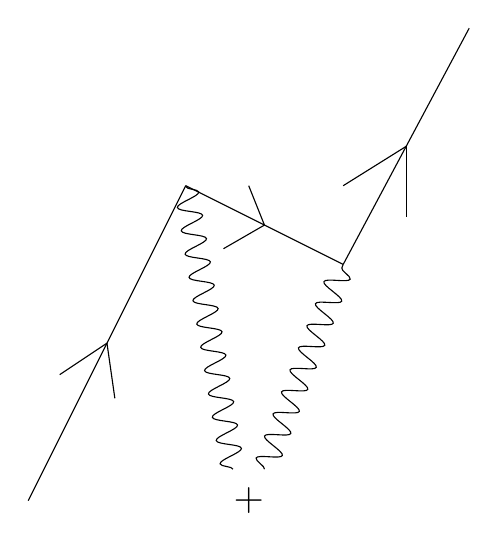
\begin{tikzpicture}[scale=2]

	%% line 1
	\draw (-1, 0) --(0,2);
	%% arrow on line 1
	\draw (-0.5, 1) -- (-0.8, 0.8);
	\draw (-0.5, 1) -- (-0.45, 0.65);

	%% line 2
	\draw (0, 2) -- (1, 1.5);
	%% arrow on line 2
	\draw (0.5,1.75) -- (0.4, 2);
	\draw (0.5,1.75) -- (0.24, 1.6);

	%% line 3
	\draw (1, 1.5) -- (1.8, 3);
	%% arrow on line 3
	\draw (1.4, 2.25) -- (1, 2);
	\draw (1.4, 2.25) -- (1.4, 1.8);

	%% pluss sign
    \node[font=\Large] at (0.4,0) {$+$};

	\draw[decorate, decoration={snake, amplitude=1.5mm, segment length=3mm}]
       (0.3,0.2) -- (0,2);
    \draw[decorate, decoration={snake, amplitude=1.5mm, segment length=3mm}]
		(0.5,0.2) --(1, 1.5);

\end{tikzpicture}
\end{center}
We can estimate the distance an electron might jump as it undergoes the process. First the time for which the virtual pair exists can be estimated from the uncertainty principle. Energy conservation is violated by $\displaystyle 2mc^2$ at least so $\displaystyle \Delta t = \frac{\hbar}{2mc^2}$ (which is approximately the reciprocal of the Zitterbewegung frequency). The distance the electron appears to jump then is of the order of $c \Delta t = \frac{\hbar c}{2mc^2} = 0.002$ angstroms. This is the approximate size of the fast back and forth motion of Zitterbewegung.


\section{The QED LaGrangian and Gauge Invariance}
The LaGrangian for electrons, photons, and the interaction between the two is the LaGrangian of Quantum ElectroDynamics.
\begin{equation}
	\mathcal{L} = -\hbar c \overline{\psi} \left( \gamma_{\mu} \frac{ \partial  }{ \partial x_{\mu} } + \frac{mc}{\hbar}  \right) \psi - \frac{1}{4}F_{\mu v} F_{\mu v} - ie \overline{\psi}\gamma_{\mu}A_{\mu}\psi
\end{equation}
QED is out first complete example on an interacting Quantum Field Theory. It taught us a great deal about the laws of physics.
\\
\\
The primary difference between Quantum Mechanics and Quantum Field Theory is that particled can be created and destroyed. The probability to find an electron or a photon integrated over space does not have to be done. It can change with time. We have written the field of the photon and the electron in terms of creation and annihilation operators.
\begin{align*}
	A_{\mu} &= \frac{1}{\sqrt{V} } \sum_{k \alpha} \sqrt{\frac{\hbar c^2}{2 \omega}} \epsilon^{(\alpha)}_{\mu} \left( a_{k, \alpha} \left( t \right) e^{i\vec{k}\cdot \vec{x}} + a^{\dagger}_{k, \alpha} \left( t \right) e^{-i \vec{k} \cdot \vec{x}} \right) \\
	\psi \left( \vec{x}, t \right) &= \sum_{\vec{p}} \sum_{s=1}^{2} \sqrt{\frac{mc^2}{EV}}  \left( b^{(s)}_{\vec{p}} u^{(s)}_{\vec{p}} e^{i\left( \vec{p} \cdot \vec{x} - Et \right) / \hbar} + d^{\left( s \right) \dagger}_{\vec{p}} v^{(s)}_{\vec{p}} e^{-i\left( \vec{p} \cdot \vec{x} - Et \right) / \hbar} \right) \\
	\psi^{\dagger}\left( \vec{x}, t \right)  &= \sum_{\vec{p}} \sum_{s=1}^{2} \sqrt{\frac{mc^2}{EV}} \left( b^{\left( s \right) \dagger}_{\vec{p}} u^{\left( s \right) \dagger}_{\vec{p}} e^{-i\left( \vec{p} \cdot \vec{x} - Et \right) / \hbar} +d^{(s)}_{\vec{p}} v^{(s)\dagger}_{\vec{p}} e^{i\left( \vec{p} \cdot \vec{x} - Et \right) / \hbar} \right) 
.\end{align*}
\\
\\
Note that in the interaction term $\displaystyle -ie \overline{\psi}\gamma_{\mu}A_{\mu}\psi$ photons can be created or destroyed singly but that electrons must be created and destroyed along with a positron.
\\
Phase (or Gauge) symmetry can be studied very simply from this LaGrangian. We have shown that the phase transformation
\begin{align*}
	\psi &\to e^{i \lambda \left( x \right)}\psi \\
	A_{\mu} \to A_{\mu} &- \frac{\hbar c}{e}\frac{ \partial \lambda \left( x \right)  }{ \partial x_{\mu} } 
.\end{align*}
leaves the Schrodinger equation invariant. This can be most directly studied using the LaGrangian. We can deduve from the above transformation that
\begin{equation}
    F_{\mu v} = \frac{ \partial A_{v} }{ \partial x_{\mu} } - \frac{ \partial A_{\mu} }{ \partial x_{v} } \to F_{\mu v} - \frac{\hbar c}{e} \left( \frac{ \partial  }{ \partial x_{\mu} } \frac{ \partial \lambda \left( x \right)  }{ \partial x_{v} } - \frac{ \partial  }{ \partial x_{v} } \frac{ \partial \lambda \left( x \right)  }{ \partial x_{\mu} }     \right)  = F_{\mu v}
\end{equation}
\\
\\
The transformed LaGrangian then can be computed easily.
\begin{equation}
	\mathcal{L} = -\hbar c \overline{\psi} \left( \gamma_{\mu} \frac{ \partial  }{ \partial x_{\mu} } + \frac{mc}{\hbar}  \right) \psi  - \frac{1}{4} F_{\mu v} F_{\mu v} - i e \overline{ \psi } \gamma_{\mu } A_{\mu} \psi
\end{equation}
The exponentials from $\displaystyle \overline{\psi}$ and $\displaystyle \psi$ cancel except for the term in which $\displaystyle \psi$ is differentiated.
\begin{equation}
	\mathcal{L} \to \mathcal{L} - i \hbar c \overline{\psi}\gamma_{\mu} \frac{ \partial \lambda }{ \partial x_{\mu} } \psi - i e \overline{\psi} \gamma_{\mu} \frac{-\hbar c}{e} \frac{ \partial \lambda }{ \partial x_{\mu} } \psi = \mathcal{L}
\end{equation}
This all may seem fairly simple but imagine that we add a mass term for the EM field, $\displaystyle -m^2 A_{\mu} a_{\mu}$. The LaGrangian is no longer guage invariant. Guage invariance implies zero mass photons and even maintains the massless photon after radiative corrections. Guage invariance also implies the existance of a conserved current. Remember that the electric current in 4D also includes the charge density. Guage invariance implies conservation of charge, another important result.
\\
\\
This simple transformation $\displaystyle \psi \to e^{i \lambda \left( x \right) }$ is called a local U(1) symmetry where the U stands for unitary.
\\
\\
The Weak interactions are based on an SU(2) symmetry. This is just a local phase symmetry times arbitrary local rotation in SU(2) space. The SU(2) group is familiar to us since angular momentum is based on SU(2). In the weak interactions, there are two particles that are symmetric (much like a spin up and a spin down electron but NOT a spin up and spin down electron). We can rotate our states into different linear combinations of the symmetric particles and the LaGrangian remains invariant. Given this local SU(2) symmetry of the fermion wave functions, we can easily deduce what boson fields are required to make the LaGrangian guage invariant. It turns out we need a triplet of bosons. (The weak interactions then get messy because of the Higgs mechanism but the underlying guage theory is still correct.)
\\
\\
The strong interactions are based on the SU(3) group. Instead of having 3 sigma matrices to do rotations in the lowest dimention representation of the group, SU(3) has eight (8) lambda matrices. The SU(3) symmetry for the quark wavefunctions require an octet of massless vector boson called gluons to make the LaGrangian guage invariant. 
\\
\\
So the standard Model is as simple as 1 2 3 in Quantum Field Theories.


\section{Interaction with a Scalar Field}
Yukawa couplings to a scalar field would be of the form $\displaystyle G \overline{\psi} \psi$ while couplings to a pseudoscalar field would be of the form $\displaystyle iG \overline{\psi} \gamma_5 \psi$.



\end{document}
